%%%%%%%%%%%%%%%%%%%%%%%%%%%%%%%%%%%%%%%%%%%%%%%%%%%%%%%%%%%%
% standard header
    \documentclass[aspectratio=169]{beamer}
    \mode<presentation>
%%%%%%%%%%%%%%%%%%%%%%%%%%%%%%%%%%%%%%%%%%%%%%%%%%%%%%%%%%%%
% color stuff
    \usetheme{AnnArbor}
    \usecolortheme[accent=blue]{solarized}
    \colorlet{solarizedMixFg}{solarizedRebase2!80!solarizedRebase0}
    \setbeamercolor{normal text}{fg=solarizedMixFg, bg=solarizedRebase02}
    \setbeamercolor{palette primary}{fg=solarizedMixFg, bg=solarizedRebase01}
    \setbeamercolor{palette secondary}{fg=solarizedMixFg, bg=solarizedRebase01}
    \setbeamercolor{palette tertiary}{fg=solarizedMixFg, bg=solarizedRebase01}
    \setbeamercolor{palette quaternary}{fg=solarizedMixFg, bg=solarizedRebase01}
%%%%%%%%%%%%%%%%%%%%%%%%%%%%%%%%%%%%%%%%%%%%%%%%%%%%%%%%%%%%
% font stuff
    \usepackage{hejohns-fonts}
    \usefonttheme{serif}
%%%%%%%%%%%%%%%%%%%%%%%%%%%%%%%%%%%%%%%%%%%%%%%%%%%%%%%%%%%%
% packages
    \usepackage{tikz}
    \usepackage{tikz-cd}
    \usetikzlibrary{positioning}
    \usepackage{graphicx}
    \usepackage{media9}
    \usepackage{svg}
%%%%%%%%%%%%%%%%%%%%%%%%%%%%%%%%%%%%%%%%%%%%%%%%%%%%%%%%%%%%
\begin{document}
%\beamertemplatenavigationsymbolsempty
\setbeamertemplate{navigation symbols}{}
%\setbeamercolor{button}{bg=blue, fg=white}
\title[Judgmental Reconstruction]{`modal logic'}
\author{hejohns}
\date{\today}
\titlegraphic{\fbox{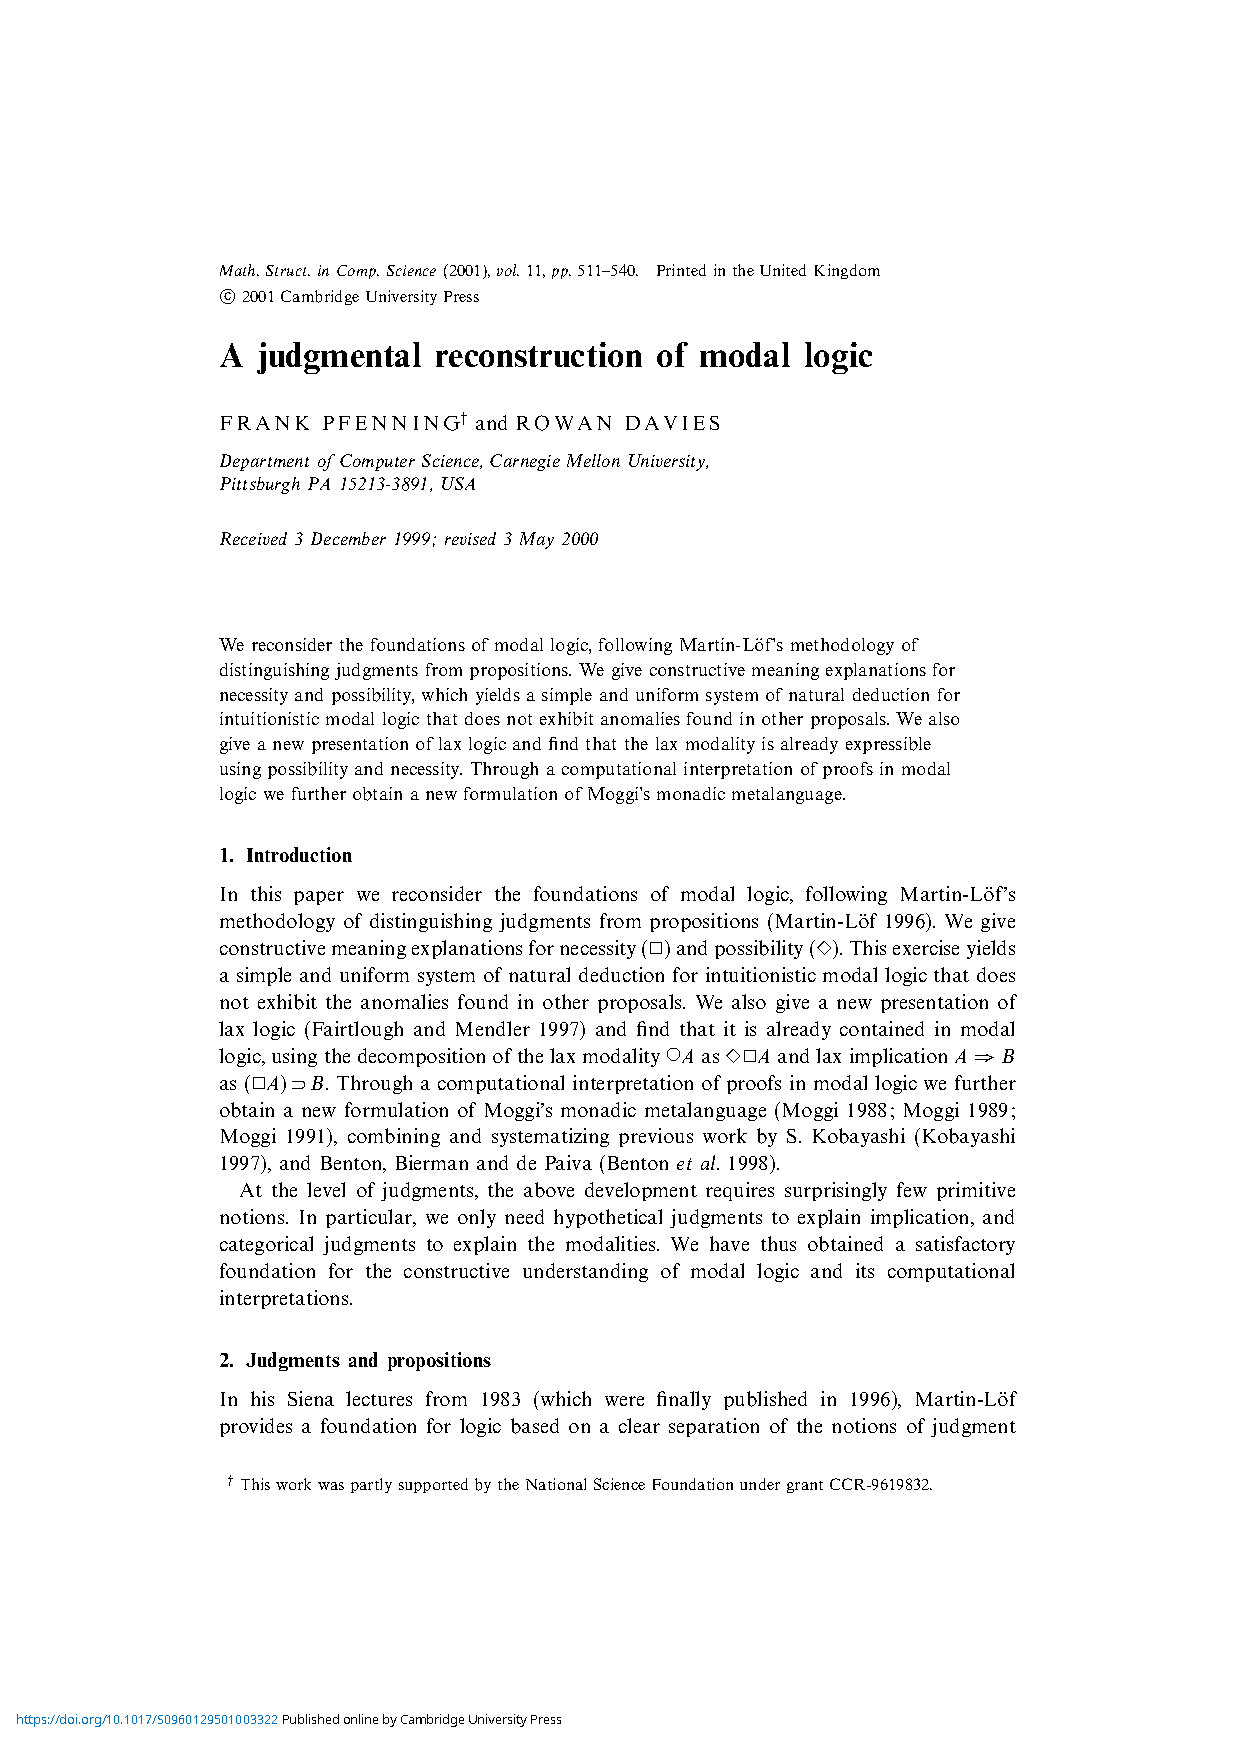
\includegraphics[page=1,scale=0.6,clip,trim=2.5cm 9cm 5.2cm 4.0cm]{jr.pdf}}}
\begin{frame}
    \titlepage
\end{frame}
\begin{frame}
    \frametitle{Outline}
    \tableofcontents
\end{frame}
\section{Pre paper}
\subsection{Pre Pre ~1960}
\begin{frame}
    \begin{itemize}
        \item prior
    \end{itemize}
\end{frame}
\subsection{Pre ~1960}
\begin{frame}
    \begin{itemize}
        \item hilbert proofs
    \end{itemize}
\end{frame}
\subsection{Kripke Semantics}
\begin{frame}
    \begin{definition}
        $\mathcal{M} = ⟨\mathcal{W}  : Set,
        R : \mathcal{W} × \mathcal{W} → 2,
        V : ω → \mathcal{W} → 2⟩$
    \end{definition}
    \begin{definition}
        \begin{align*}
            &⊨^{\mathcal{M}}_{α ∈ \mathcal{W}} P_n ⟺ V(n)(α) \\
            &⊨^{\mathcal{M}}_{α ∈ \mathcal{W}} ⊥ ⟺ false \\
            &⊨^{\mathcal{M}}_{α ∈ \mathcal{W}} A \land B ⟺ ⊨^{\mathcal{M}}_α A~and~⊨^{\mathcal{M}}_{α} B\\
            &⊨^{\mathcal{M}}_{α ∈ \mathcal{W}} A \lor B ⟺ ⊨^{\mathcal{M}}_α A~or~⊨^{\mathcal{M}}_{α} B\\
            &⊨^{\mathcal{M}}_{α ∈ \mathcal{W}} A → B ⟺ ⊨^{\mathcal{M}}_α A ⟹ ⊨^{\mathcal{M}}_{α} B\\
            &⊨^{\mathcal{M}}_{α ∈ \mathcal{W}} \Box A ⟺ ∀β∈\mathcal{W}.αRβ ⟹ ⊨^{\mathcal{W}}_{β} A \\
            &⊨^{\mathcal{M}}_{α ∈ \mathcal{W}} \Diamond A ⟺ ∃β∈\mathcal{W}.αRβ \land ⊨^{\mathcal{W}}_{β} A \\
        \end{align*}
    \end{definition}
\end{frame}
\begin{frame}
    \begin{definition}
        $\mathcal{M} = ⟨\mathcal{W}  : Set,
        ≤,
        V : ω → \mathcal{W} → 2⟩$ \\
        $α≤β ⟹ ⊨^{\mathcal{M}}_α P_n ⟹ ⊨^{\mathcal{M}}_β P_n$
    \end{definition}
    \begin{definition}
        \begin{align*}
            &⊨^{\mathcal{M}}_α A → B ⟺ ∀β.α≤β ⟹ ⊨^{\mathcal{M}}_β A ⟹ ⊨^{\mathcal{M}}_β B \\
        \end{align*}
    \end{definition}
\end{frame}
\begin{frame}
    $\Box(A → B)$
\end{frame}
%\begin{frame}
%    \begin{tikzpicture}[commutative diagrams/.cd, every diagram, scale=4]
%        \begin{scope}[node distance=1 and 1]
%            \node[](K) at (0, 0){K$};
%            \node[above=of K](D){$D$};
%            \node[above=of D](M){$M$};
%            \node[above right=0.6 and 0.2 of K](K4){$K4$};
%            \node[above right=0.2 and 0.9 of K](K5){$K5$};
%            \node[above right=0.1 and 0.45 of K5](K45){$K45$};
%            \node[above=of K4](D4){$D4$};
%            \node[above=of D4](S4){$S4=M4$};
%            \node[right=2 of K](KB){$KB$};
%            \node[above right=0.6 and 0.2 of KB](KB5){$KB5$};
%        \end{scope}
%        \draw[commutative diagrams/.cd, every label]
%        (D)edge(M)
%        (K)edge(D)
%        (K)edge(K4)
%        (K)edge(KB)
%        ;
%    \end{tikzpicture}
%\end{frame}
\section{Pfenning, Davies}
\subsection{Judgment, in passing}
\begin{frame}
    \frametitle{Judgment}
    \begin{itemize}
        \item ``Of course, there would be needed here an analysis of what is understood by an expression, but that is a comparatively trivial matter, as compared with explaining the notion of proposition and judgement.
            An expression in the  most general sense of the word is nothing but a form, that is, something that we can passively recognize as the same in its manifold occurrences and actively reproduce in many copies.
            But I think that I shall have to rely here upon an agreement that we have such a general notion of expression, which is formal in character, so that the rule can now count as a formal rule."
    \end{itemize}
\end{frame}
\begin{frame}
    \frametitle{Local Soundness/Completeness}
\end{frame}
\section*{References}
\begin{frame}[allowframebreaks]
    \frametitle{References}
    \begin{thebibliography}{00}
        \setbeamertemplate{bibliography item}{\insertbiblabel}
        \bibitem{sourceA}
        TODO: ask me
    \end{thebibliography}
\end{frame}
\end{document}
